\documentclass[aspectratio=169, 11pt]{beamer}

% --- Packages & Setup (university template, case_1_research_project/1_presentation.tex) ---
\usepackage[utf8]{inputenc}
\usepackage[T1]{fontenc}
\usepackage{helvet}
\renewcommand{\familydefault}{\sfdefault}
\usepackage{xcolor}
\usepackage{booktabs}
\usepackage{array}
\usepackage{colortbl}
\usepackage{graphicx}
\usepackage{tikz}
\usetikzlibrary{calc,positioning,arrows.meta,shapes.geometric}
\usepackage{adjustbox}
\usepackage{pifont}

\graphicspath{{figures/}{figures/dashboard/}{./}}

% --- Branding Colors ---
\definecolor{amritaMaroon}{HTML}{A4123F}
% one colour per part of the system, used the same way on every slide
\definecolor{cTraffic}{HTML}{1E40AF}
\definecolor{cTrust}{HTML}{6B21A8}
\definecolor{cVerify}{HTML}{B45309}
\definecolor{cDissem}{HTML}{166534}
\definecolor{cRSU}{HTML}{991B1B}
\definecolor{inkGray}{HTML}{4B5563}
\definecolor{baseBlue}{HTML}{1F5FA0}
\colorlet{rowBase}{baseBlue!12}
\colorlet{rowProp}{amritaMaroon!12}

% --- Theme Setup ---
\usetheme{Madrid}
\usecolortheme[named=amritaMaroon]{structure}
\setbeamertemplate{navigation symbols}{}
\setbeamertemplate{footline}[frame number]
\setbeamerfont{frametitle}{series=\bfseries}
\setbeamertemplate{bibliography item}[text]
\setbeamerfont{bibliography item}{size=\fontsize{7.6}{8.9}\selectfont}
\setbeamerfont{bibliography entry author}{size=\fontsize{7.6}{8.9}\selectfont}
\setbeamerfont{bibliography entry title}{size=\fontsize{7.6}{8.9}\selectfont}
\setbeamerfont{bibliography entry location}{size=\fontsize{7.6}{8.9}\selectfont}
\setbeamerfont{bibliography entry note}{size=\fontsize{7.6}{8.9}\selectfont}
% beamer starts every reference with an empty 1.5em-high box; make it zero so 19 references fit on two slides
\makeatletter
\patchcmd{\beamer@newblock}{\ht\beamer@tempbox=1.5em}{\ht\beamer@tempbox=0pt}{}{}
\makeatother
\let\origthebibliography\thebibliography
\renewcommand{\thebibliography}[1]{\origthebibliography{#1}\setlength{\itemsep}{1.5pt}\setlength{\parskip}{0pt}}
\hyphenpenalty=10000
\exhyphenpenalty=10000


% =====================================================
% SHARED PROJECT DETAILS — REPORT AND PRESENTATION
% =====================================================

\newcommand{\ProjectTitle}{Trust-Aware Clustering and Controlled Broadcast for Secure IoV Communication}

\newcommand{\CourseLine}{23CSE498 -- Project Phase II (External Review)}

\newcommand{\TeamNumber}{83}

% Team Members
\newcommand{\RegA}{CB.SC.U4CSE23650}
\newcommand{\StudentA}{Akhil Rudrapaka}

\newcommand{\RegB}{CB.SC.U4CSE23620}
\newcommand{\StudentB}{G Nikshith}

\newcommand{\RegC}{CB.SC.U4CSE23332}
\newcommand{\StudentC}{K Charan}

\newcommand{\RegD}{CB.SC.U4CSE23640}
\newcommand{\StudentD}{P Sreeshanth}

\newcommand{\RegE}{CB.SC.U4CSE23625}
\newcommand{\StudentE}{K Chakri}

% Project Guide
\newcommand{\GuideName}{Dr. Radhika G}
\newcommand{\GuideDesignation}{Department of CSE}
\newcommand{\GuideInstitution}{Amrita Vishwa Vidyapeetham}

% Project Classification
\newcommand{\ProjectType}{Type 1 -- Research-Based Project}

% Repository
\newcommand{\RepoURL}{github.com/AkhilRudrapaka/IoV-Emergency-Broadcast}

% Generated by scripts/make_figures_and_tables.py from results/urban/processed and results/urban/sensitivity.
% 200 vehicles unless the name says FiveH (500) or Fifty (50). Do not edit by hand.
\newcommand{\NFrFlood}{185.8}
\newcommand{\NFrFloodRad}{186.0}
\newcommand{\NFrSlot}{54.7}
\newcommand{\NFrSlotRad}{24.1}
\newcommand{\NFrProp}{26.4}
\newcommand{\NFrRoute}{10.8}
\newcommand{\NFrPropFiveH}{31.3}
\newcommand{\NFrFloodFiveH}{451.6}
\newcommand{\NFrSlotRadFiveH}{31.9}
\newcommand{\NFrSlotFiveH}{152.2}
\newcommand{\NFrPropFifty}{18.4}
\newcommand{\NFrFloodFifty}{50.7}
\newcommand{\NCutVsFlood}{86}
\newcommand{\NCutVsSlot}{52}
\newcommand{\NLossFlood}{9632}
\newcommand{\NLossSlot}{2070}
\newcommand{\NLossSlotRad}{188}
\newcommand{\NLossProp}{151}
\newcommand{\NLossPropFiveH}{559}
\newcommand{\NLossSlotRadFiveH}{1405}
\newcommand{\NTnFlood}{31.8}
\newcommand{\NTnSlotRad}{34.0}
\newcommand{\NTnProp}{35.3}
\newcommand{\NTnSlot}{32.5}
\newcommand{\NDTnFlood}{+3.5}
\newcommand{\NDTnFloodCI}{1.7}
\newcommand{\NDTnSlotRadFiveH}{+9.4}
\newcommand{\NDTnSlotRadFiveHCI}{2.2}
\newcommand{\NDTnSlotRadFifty}{$-$6.7}
\newcommand{\NDTnSlotRadFiftyCI}{3.9}
\newcommand{\NDFrSlotRad}{+2.3}
\newcommand{\NDFrSlotRadCI}{1.6}
\newcommand{\NSupProp}{89.1}
\newcommand{\NSupSlotRad}{90.4}
\newcommand{\NSupSlot}{73.3}
\newcommand{\NReachSlotRadFifty}{95.7}
\newcommand{\NReachSlotFifty}{91.5}
\newcommand{\NReachFloodTwoH}{99.9}
\newcommand{\NRsuProp}{21.4}
\newcommand{\NRsuFlood}{22.0}
\newcommand{\NRsuRoute}{30.5}
\newcommand{\NRsuRouteRuns}{28}
\newcommand{\NQuorumMs}{12.1}
\newcommand{\NFrNoSec}{19.6}
\newcommand{\NTnNoSec}{8.0}
\newcommand{\NSecFrames}{6.9}
\newcommand{\NSecTn}{27.3}
\newcommand{\NFrNoClu}{46.1}
\newcommand{\NFrNoCluFiveH}{215.5}
\newcommand{\NFrNoCov}{186.0}
\newcommand{\NFrNoRad}{40.6}
\newcommand{\NForgNoVote}{30}
\newcommand{\NForgVoteOnly}{26}
\newcommand{\NForgFull}{0}
\newcommand{\NForgOnOffHalf}{0}
\newcommand{\NForgOnOffNine}{25}
\newcommand{\NForgCertFull}{26}
\newcommand{\NRuns}{30}
\newcommand{\NScenarios}{180}
\newcommand{\NDensities}{6}
\newcommand{\NFrNoSlots}{34.1}
\newcommand{\NFrNoCluFwd}{49.9}
\newcommand{\NFrNoRep}{24.7}
\newcommand{\NFrPropPlusRoute}{37.2}
\newcommand{\NDTnFloodRad}{+3.9}
\newcommand{\NDTnFloodRadCI}{1.3}
\newcommand{\NDTnSlot}{+2.8}
\newcommand{\NDTnSlotCI}{1.7}
\newcommand{\NDTnSlotRad}{+1.3}
\newcommand{\NDTnSlotRadCI}{1.9}
\newcommand{\NDTnSlotRadThreeH}{+3.4}
\newcommand{\NDTnSlotRadThreeHCI}{1.5}
\newcommand{\NDFrSlot}{$-$28.2}
\newcommand{\NDFrSlotCI}{4.8}
\newcommand{\NDFrSlotRadHundred}{+2.1}
\newcommand{\NDFrSlotRadHundredCI}{1.6}
\newcommand{\NDLossSlotRad}{$-$36}
\newcommand{\NDLossSlotRadCI}{55}
\newcommand{\NDLossSlotRadFiveH}{$-$846}
\newcommand{\NDLossSlotRadFiveHCI}{554}
\newcommand{\NDLossSlotRadHundred}{+33}
\newcommand{\NDLossSlotRadHundredCI}{25}
\newcommand{\NDReachSlotRadFifty}{+4.3}
\newcommand{\NDReachSlotRadFiftyCI}{4.1}
\newcommand{\NDRsuSlotRad}{+0.9}
\newcommand{\NDRsuSlotRadCI}{0.5}
\newcommand{\NNTnSlotRadFifty}{27}
\newcommand{\NTnSlotRadFifty}{44.3}
\newcommand{\NTnPropFifty}{37.8}
\newcommand{\NTnPropFiveH}{40.7}
\newcommand{\NTnSlotRadFiveH}{31.3}
\newcommand{\NRsuSlotRad}{20.5}

% Generated by scripts/make_slide_assets.py; numbers used only by the presentation
\newcommand{\NReachProp}{100.0}

\newcommand{\gentable}[1]{\begin{adjustbox}{max width=\textwidth}\input{generated/#1}\end{adjustbox}}

% ---------------------------------------------------------------- reusable slide elements
% the one message of a slide, at its foot
\newcommand{\takeaway}[1]{\par\vfill\noindent
  \tikz\node[fill=amritaMaroon!8, draw=amritaMaroon!55, rounded corners=2pt, inner sep=6pt,
             text width=\dimexpr\textwidth-14pt\relax, font=\small, align=left]{#1};\par}
% short grey caption
\newcommand{\shotcap}[1]{\par\vspace{2pt}{\footnotesize\color{inkGray}#1\par}}
% a point: coloured heading, one line of explanation
\newcommand{\point}[3]{\par\noindent{\color{#1}\textbf{#2}}\par\noindent #3\par\vspace{8pt}}
% an image with annotations in image coordinates: (0,0) bottom left, (1,1) top right
\newcommand{\annot}[3]{\begin{tikzpicture}
  \node[inner sep=0pt, anchor=south west] (I) at (0,0) {\includegraphics[#1]{#2}};
  \begin{scope}[x={(I.south east)}, y={(I.north west)}] #3 \end{scope}\end{tikzpicture}}
\newcommand{\yes}{{\color{cDissem}\ding{51}}}
\newcommand{\no}{{\color{cRSU}\ding{55}}}
\newcommand{\plus}{{\color{cDissem}\textbf{+}}}
\newcommand{\minus}{{\color{cRSU}\textbf{$-$}}}

\tikzset{
  tile/.style={draw=#1, fill=#1!7, line width=0.8pt, rounded corners=3pt, inner sep=5pt, align=center},
  flow/.style={-{Stealth[length=6pt]}, line width=1.2pt, color=inkGray},
  num/.style={circle, fill=#1, text=white, font=\footnotesize\bfseries, inner sep=1.5pt, minimum size=0.52cm},
  call/.style={draw=amritaMaroon, fill=white, rounded corners=1.5pt, inner sep=2.2pt, font=\scriptsize\bfseries,
               text=amritaMaroon, align=center},
  ptr/.style={amritaMaroon, line width=0.9pt},
  hl/.style={amritaMaroon, line width=1.2pt},
  car/.style={draw=black!55, fill=black!25, rounded corners=1pt, minimum width=0.32cm, minimum height=0.17cm,
              inner sep=0pt},
  src/.style={draw=red!50!black, fill=red!80, rounded corners=1pt, minimum width=0.32cm, minimum height=0.17cm,
              inner sep=0pt},
  objective/.style={draw=amritaMaroon!70, fill=amritaMaroon!4, line width=0.7pt, rounded corners=3pt, inner sep=7pt,
                    text width=4.0cm, minimum height=2.8cm, align=center, anchor=north west},
  idea/.style={tile=#1, text width=2.2cm, minimum height=3.95cm, anchor=north, font=\small},
  chal/.style={draw=#1, fill=#1!6, line width=0.8pt, rounded corners=3pt, inner sep=7pt, text width=3.75cm,
               minimum height=2.4cm, align=center, anchor=north},
  goal/.style={draw=#1, fill=#1!6, rounded corners=2pt, text width=2.75cm, minimum height=1.45cm, align=left,
               font=\small, inner sep=4pt, anchor=north west},
  gapbox/.style={draw=#1, fill=#1!6, line width=0.8pt, rounded corners=3pt, text width=3.0cm, minimum height=3.1cm,
                 align=left, inner sep=5pt, anchor=north west, font=\small},
  chip/.style={draw=#1, fill=#1!10, line width=0.8pt, rounded corners=2pt, text width=2.65cm, minimum height=0.95cm,
               align=center, font=\small\bfseries, text=#1, inner sep=3pt},
  pipe/.style={tile=#1, text width=2.0cm, minimum height=1.55cm, font=\small},
  metric/.style={draw=#1, fill=#1!5, line width=0.6pt, rounded corners=2pt, text width=2.35cm, align=center,
                 font=\small, inner sep=4pt, anchor=north west},
  quad/.style={draw=#1, fill=#1!5, line width=0.7pt, rounded corners=3pt, inner sep=7pt, text width=6.5cm,
               minimum height=2.75cm, align=left, anchor=north west, font=\small},
  step/.style={tile=#1, text width=4.9cm, align=left, font=\small, anchor=north},
  finding/.style={draw=#1, fill=#1!6, rounded corners=3pt, inner sep=6pt, text width=3.95cm, minimum height=2.0cm,
                  align=left, anchor=north west, font=\small},
}

\begin{document}

% =========================================================================
% TITLE SLIDE (Research-Based Project)
% =========================================================================
\begin{frame}
    \begin{tikzpicture}[remember picture,overlay]
        \node[fill=amritaMaroon, text=white, font=\bfseries\footnotesize, anchor=north east, rounded corners=2pt, inner sep=5pt]
        at ($(current page.north east) + (-0.2cm,-0.2cm)$)
        {Type 1: Research Project};
    \end{tikzpicture}

    \centering
    
\includegraphics[width=2.7cm]{logo.png}\par\vspace{0.12cm}
    {\Large \textbf{\textcolor{amritaMaroon}{Emergency Message Dissemination for Broadcast Storm\\[1pt]
    Mitigation in the Internet of Vehicles}}}\par\vspace{0.1cm}
    {\color{amritaMaroon}\rule{0.55\textwidth}{0.8pt}}\par\vspace{0.06cm}
    {\small \textbf{\CourseLine} \quad | \quad \textbf{Team Number: \TeamNumber}}\par\vspace{0.18cm}

    {\small
    \renewcommand{\arraystretch}{1.1}
    \begin{tabular}{|c|c|l|}
        \hline
        \rowcolor{amritaMaroon}\textcolor{white}{\textbf{S.No}} & \textcolor{white}{\textbf{Register Number}} &
        \textcolor{white}{\textbf{Student Name}} \\
        \hline
        1 & \RegA & \StudentA \\ \hline
        2 & \RegB & \StudentB \\ \hline
        3 & \RegC & \StudentC \\ \hline
        4 & \RegD & \StudentD \\ \hline
        5 & \RegE & \StudentE \\ \hline
    \end{tabular}}\par\vspace{0.18cm}

    {\small Guide: \textbf{\GuideName}, \GuideDesignation, \GuideInstitution}\par\vspace{0.05cm}
    {\footnotesize \today}
\end{frame}

% =========================================================================
% GUIDE APPROVAL (the screenshot is shown exactly as received)
% =========================================================================
\begin{frame}{2. Guide Approval}
    \centering
    \vspace{0.05cm}
    {\setlength{\fboxsep}{0pt}\fcolorbox{inkGray!40}{white}{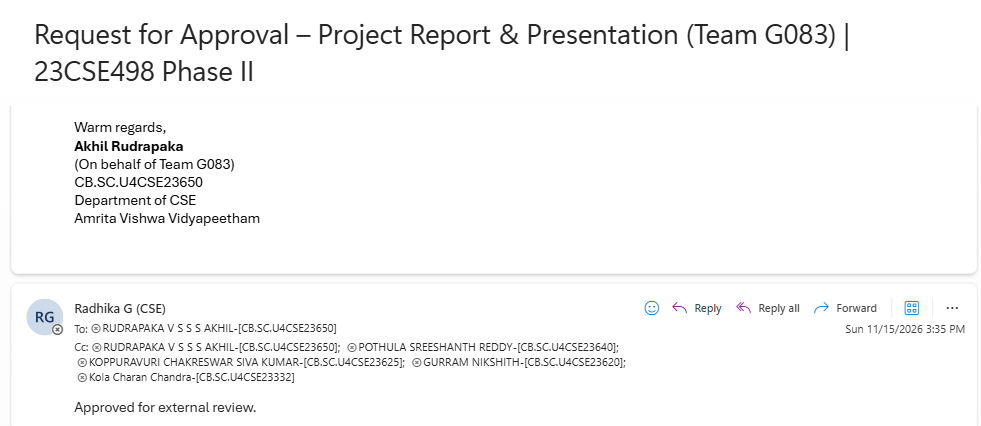
\includegraphics[width=0.93\textwidth]{guide_approval_email.png}}}
    \par\vspace{8pt}
    {\small Reply from the project guide, \textbf{\GuideName}, to the team's request for approval of the project report
    and presentation: \textbf{\color{cDissem}``Approved for external review.''}}
\end{frame}

% =========================================================================
\section{Introduction}

\begin{frame}{3. Introduction: The Internet of Vehicles}
    \begin{columns}[c]
        \column{0.55\textwidth}
        \centering
        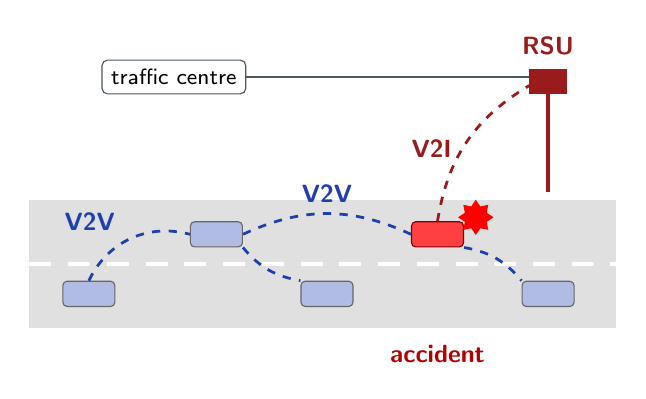
\begin{tikzpicture}[x=1.08cm,y=1.08cm,
            veh/.style={draw=black!60, fill=cTraffic!35, rounded corners=1.5pt, minimum width=0.66cm,
                        minimum height=0.32cm, inner sep=0pt},
            wave/.style={cTraffic, line width=1pt, dashed},
            lab/.style={font=\small\bfseries}]
            \fill[black!12] (0,0) rectangle (6.9,1.5);
            \draw[white, line width=1.2pt, dash pattern=on 8pt off 6pt] (0,0.75) -- (6.9,0.75);
            \node[veh] (a) at (0.7,0.4) {};
            \node[veh] (b) at (2.2,1.1) {};
            \node[veh] (c) at (3.5,0.4) {};
            \node[veh, fill=red!75, draw=red!50!black] (d) at (4.8,1.1) {};
            \node[veh] (e) at (6.1,0.4) {};
            \node[star, star points=8, fill=red, inner sep=1pt, minimum size=0.45cm] at (5.25,1.3) {};
            \node[font=\small\bfseries, text=red!70!black] at (4.8,-0.3) {accident};
            \draw[wave] (a.north) to[bend left=40] node[pos=0.45, above left, lab, text=cTraffic] {V2V} (b.west);
            \draw[wave] (b.south east) to[bend right=20] (c.north west);
            \draw[wave] (d.west) to[bend right=25] node[midway, above, lab, text=cTraffic] {V2V} (b.east);
            \draw[wave] (d.south east) to[bend left=20] (e.north west);
            \draw[cRSU, line width=1.5pt] (6.1,1.6) -- (6.1,2.75);
            \fill[cRSU] (5.88,2.75) rectangle (6.32,3.05);
            \node[lab, text=cRSU] at (6.1,3.32) {RSU};
            \draw[wave, cRSU] (d.north) to[bend left=25] node[pos=0.45, left, lab, text=cRSU] {V2I} (5.88,2.85);
            \node[draw=inkGray, fill=white, rounded corners=2pt, font=\footnotesize, align=center] (tc) at (1.7,2.95)
                {traffic centre};
            \draw[inkGray, line width=1pt] (tc.east) -- (5.88,2.95);
        \end{tikzpicture}
        \column{0.43\textwidth}
        \point{cTraffic}{Vehicle to vehicle (V2V)}{Nearby vehicles share short radio messages directly.}
        \point{cRSU}{Vehicle to roadside unit (V2I)}{Roadside units (RSUs) pass messages to the traffic centre.}
        \point{amritaMaroon}{Emergency alerts}{After a crash, vehicles behind must know within milliseconds.}
    \end{columns}
    \takeaway{\textbf{Our focus:} spreading an accident alert quickly, with few copies, and only if it is genuine.}
\end{frame}

\begin{frame}{4. The Real-World Problem: One Accident, Too Many Copies}
    \begin{columns}[T]
        \column{0.55\textwidth}
        \centering
        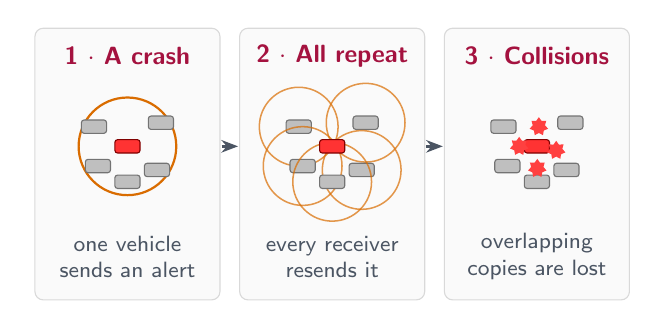
\begin{tikzpicture}[x=1cm,y=1cm,
            ptitle/.style={font=\small\bfseries, text=amritaMaroon, align=center, text width=2.3cm},
            pnote/.style={font=\footnotesize, text=inkGray, align=center, text width=2.25cm}]
            \foreach \x in {0,2.6,5.2} \draw[black!15, rounded corners=3pt, fill=black!2] (\x,0) rectangle (\x+2.35,3.45);
            \node[ptitle] at (1.175,3.1) {1 $\cdot$ A crash};
            \draw[orange!85!black, line width=0.8pt] (1.175,1.95) circle (0.62);
            \foreach \x/\y in {0.75/2.2, 1.6/2.25, 0.8/1.7, 1.55/1.65, 1.175/1.5} \node[car] at (\x,\y) {};
            \node[src] at (1.175,1.95) {};
            \node[pnote] at (1.175,0.55) {one vehicle sends an alert};
            \node[ptitle] at (3.775,3.1) {2 $\cdot$ All repeat};
            \foreach \x/\y in {3.35/2.2, 4.2/2.25, 3.4/1.7, 4.15/1.65, 3.775/1.5}{
                \draw[orange!85!black, line width=0.55pt, opacity=0.7] (\x,\y) circle (0.5);
                \node[car] at (\x,\y) {};}
            \node[src] at (3.775,1.95) {};
            \node[pnote] at (3.775,0.55) {every receiver resends it};
            \node[ptitle] at (6.375,3.1) {3 $\cdot$ Collisions};
            \foreach \x/\y in {5.95/2.2, 6.8/2.25, 6.0/1.7, 6.75/1.65, 6.375/1.5} \node[car] at (\x,\y) {};
            \node[src] at (6.375,1.95) {};
            \foreach \x/\y in {6.15/1.95, 6.62/1.9, 6.38/1.67, 6.4/2.2}
                \node[star, star points=7, fill=red!75, inner sep=0.4pt, minimum size=0.24cm] at (\x,\y) {};
            \node[pnote] at (6.375,0.55) {overlapping copies are lost};
            \draw[flow] (2.37,1.95) -- (2.58,1.95);
            \draw[flow] (4.97,1.95) -- (5.18,1.95);
        \end{tikzpicture}
        \par\vspace{8pt}
        \tikz\node[draw=orange!80!black, fill=orange!6, rounded corners=3pt, inner sep=6pt, text width=7.0cm,
            align=center]{\small Blind flooding, 200 vehicles, one alert (our simulation):\\[2pt]
            {\Large\textbf{\NFrFlood}} {\small frames sent} \qquad {\Large\textbf{\NLossFlood}} {\small lost receptions}};
        \column{0.43\textwidth}
        {\large\textbf{\color{amritaMaroon}Impact}}\par\vspace{6pt}
        \renewcommand{\arraystretch}{1.5}
        \begin{tabular}{@{}>{\bfseries\raggedright\arraybackslash}p{2.3cm}>{\raggedright\arraybackslash}p{3.6cm}@{}}
            Duplicates & most vehicles already have it \\
            Congestion & one shared radio channel \\
            Collisions & copies are lost \\
            Delay & a busy channel is slow \\
            Fake alerts & spread just as fast \\
        \end{tabular}
        \par\vspace{6pt}
        {\footnotesize\color{inkGray} This is the ``broadcast storm'' \cite{ni1999broadcast}.}
    \end{columns}
\end{frame}

\begin{frame}{5. Problem Statement}
    \centering
    \vspace{0.15cm}
    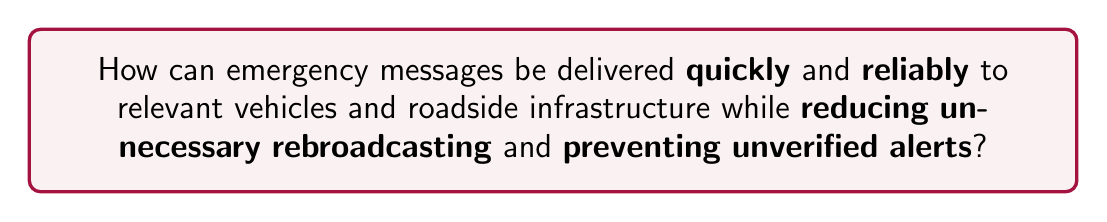
\begin{tikzpicture}
        \node[draw=amritaMaroon, line width=1.2pt, fill=amritaMaroon!6, rounded corners=4pt, inner sep=10pt,
              text width=12.6cm, align=center, font=\large] {How can emergency messages be delivered \textbf{quickly}
              and \textbf{reliably} to relevant vehicles and roadside infrastructure while \textbf{reducing unnecessary
              rebroadcasting} and \textbf{preventing unverified alerts}?};
    \end{tikzpicture}
    \par\vspace{0.45cm}
    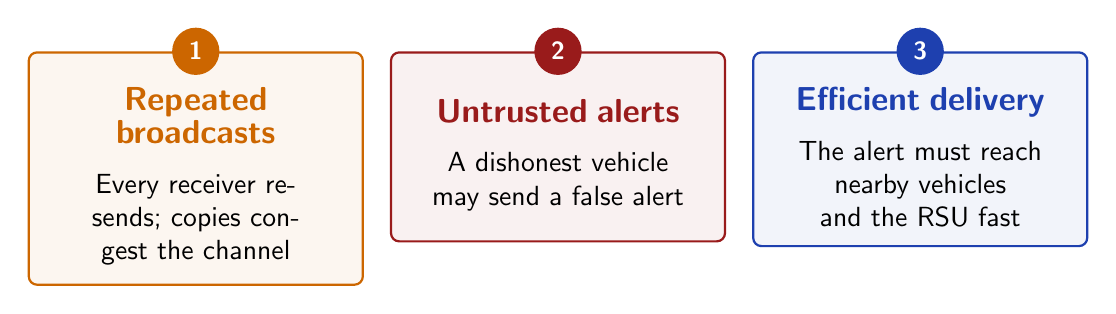
\begin{tikzpicture}[x=1cm,y=1cm]
        \foreach \i/\x/\c/\t/\b in {1/0/orange!80!black/{Repeated broadcasts}/{Every receiver resends; copies congest
              the channel},
            2/4.6/cRSU/{Untrusted alerts}/{A dishonest vehicle may send a false alert},
            3/9.2/cTraffic/{Efficient delivery}/{The alert must reach nearby vehicles and the RSU fast}}{
            \node[chal=\c] (k\i) at (\x,0) {\mbox{}\\[2pt]{\large\textbf{\color{\c}\t}}\\[6pt]\b};
            \node[circle, fill=\c, text=white, font=\small\bfseries, minimum size=0.6cm, inner sep=0pt] at (k\i.north) {\i};}
    \end{tikzpicture}
\end{frame}

\begin{frame}{6. Research Motivation}
    \begin{columns}[c]
        \column{0.5\textwidth}
        \centering
        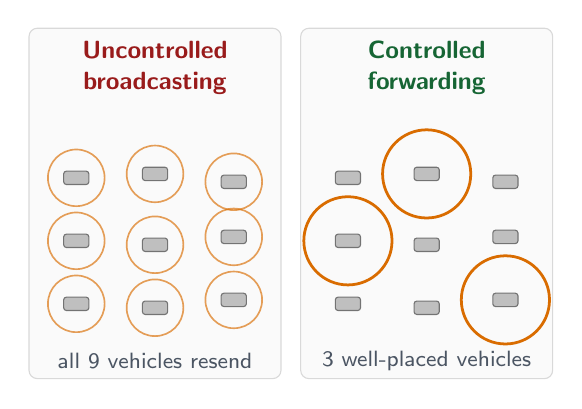
\begin{tikzpicture}[x=1cm,y=1cm,
            ring/.style={orange!85!black, line width=0.6pt},
            ptitle/.style={font=\small\bfseries, align=center, text width=3.0cm}]
            \foreach \ox/\ttl/\clr/\lab in {0/{Uncontrolled\\broadcasting}/cRSU/{all 9 vehicles resend},
                3.45/{Controlled\\forwarding}/cDissem/{3 well-placed vehicles}}{
                \draw[black!15, rounded corners=3pt, fill=black!2] (\ox,0) rectangle (\ox+3.2,4.45);
                \node[ptitle, text=\clr] at (\ox+1.6,3.95) {\ttl};
                \node[font=\footnotesize, text=inkGray] at (\ox+1.6,0.22) {\lab};
                \foreach \x/\y in {0.6/2.55, 1.6/2.6, 2.6/2.5, 0.6/1.75, 1.6/1.7, 2.6/1.8, 0.6/0.95, 1.6/0.9, 2.6/1.0}
                    \node[car] at (\ox+\x,\y) {};}
            \foreach \x/\y in {0.6/2.55, 1.6/2.6, 2.6/2.5, 0.6/1.75, 1.6/1.7, 2.6/1.8, 0.6/0.95, 1.6/0.9, 2.6/1.0}
                \draw[ring, opacity=0.65] (\x,\y) circle (0.36);
            \foreach \x/\y in {1.6/2.6, 0.6/1.75, 2.6/1.0} \draw[ring, line width=1pt] (3.45+\x,\y) circle (0.56);
        \end{tikzpicture}
        \column{0.48\textwidth}
        {\large\textbf{\color{amritaMaroon}A good alert scheme balances}}\par\vspace{6pt}
        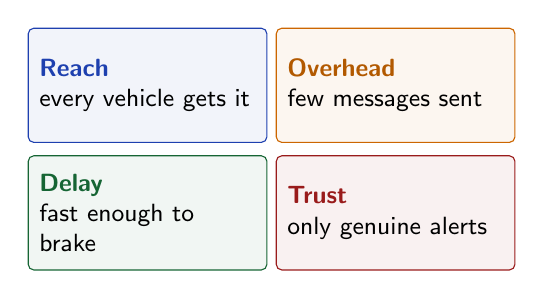
\begin{tikzpicture}[x=1cm,y=1cm]
            \node[goal=cTraffic] at (0,0) {\textbf{\color{cTraffic}Reach}\\every vehicle gets it};
            \node[goal=orange!80!black] at (3.15,0) {\textbf{\color{orange!70!black}Overhead}\\few messages sent};
            \node[goal=cDissem] at (0,-1.62) {\textbf{\color{cDissem}Delay}\\fast enough to brake};
            \node[goal=cRSU] at (3.15,-1.62) {\textbf{\color{cRSU}Trust}\\only genuine alerts};
        \end{tikzpicture}
        \par\vspace{6pt}
        Fewer copies can lower reach; checking alerts adds delay.
    \end{columns}
    \takeaway{\textbf{Motivation:} achieve all four together, and measure the trade-offs on the same traffic.}
\end{frame}

% =========================================================================
\section{Literature and Research Gap}

\begin{frame}{7. Literature Survey: Existing Approaches}
    \centering
    \small
    \setlength{\tabcolsep}{4pt}
    \renewcommand{\arraystretch}{1.08}
    \begin{tabular}{@{}>{\raggedright\arraybackslash}m{2.45cm}>{\raggedright\arraybackslash}m{7.75cm}>{\raggedright\arraybackslash}m{3.25cm}@{}}
        \toprule
        \textbf{Research area} & \textbf{Technique, in simple terms} & \textbf{Result} \\
        \midrule
        {\color{cDissem}\textbf{Broadcast suppression}} &
            \textbullet~\textbf{Probabilistic:} resend with a probability \cite{ni1999broadcast}\newline
            \textbullet~\textbf{Distance-based:} farthest vehicles go first \cite{wisitpongphan2007,korkmaz2004umb}\newline
            \textbullet~\textbf{Topology-aware:} wait while disconnected \cite{tonguz2010dvcast} &
            \plus\ fewer duplicates\newline \minus\ no alert check \\
        \midrule
        {\color{cRSU}\textbf{Trust and authentication}} &
            \textbullet~\textbf{Event trust:} combine several reports \cite{raya2008datacentric}\newline
            \textbullet~\textbf{Batch checks:} verify signatures at once \cite{zhang2008batch,naskar2025auth}\newline
            \textbullet~\textbf{Trust routing:} vehicles watch neighbours \cite{azizi2024rtrv} &
            \plus\ spots bad senders\newline \minus\ no repeat control \\
        \midrule
        {\color{cTrust}\textbf{Vehicle clustering}} &
            \textbullet~DBSCAN groups and scores vehicles \cite{chen2024dnov} &
            \plus\ stable groups\newline \minus\ no alert security \\
        \midrule
        {\color{cTraffic}\textbf{Route-based delivery}} &
            \textbullet~Route chosen by travel direction \cite{kaur2024route} &
            \plus\ less flooding\newline \minus\ no confirmation \\
        \bottomrule
    \end{tabular}
\end{frame}

\begin{frame}{8. Research Gap}
    \centering
    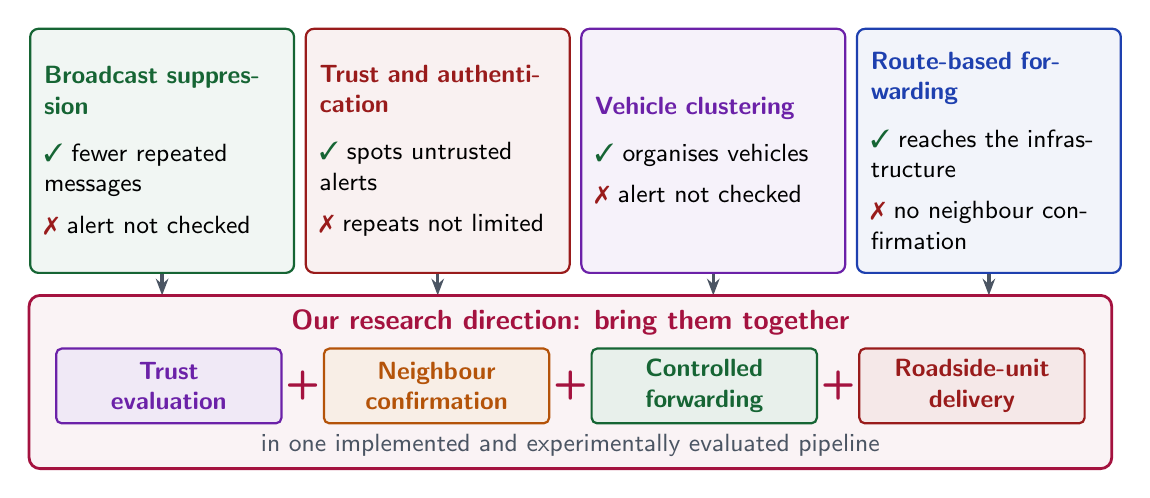
\begin{tikzpicture}[x=1cm,y=1cm]
        \foreach \i/\c/\t/\ok/\gap in {
            0/cDissem/{Broadcast suppression}/{fewer repeated messages}/{alert not checked},
            1/cRSU/{Trust and authentication}/{spots untrusted alerts}/{repeats not limited},
            2/cTrust/{Vehicle clustering}/{organises vehicles}/{alert not checked},
            3/cTraffic/{Route-based forwarding}/{reaches the infrastructure}/{no neighbour confirmation}}{
            \node[gapbox=\c] (g\i) at (3.5*\i,0) {{\color{\c}\textbf{\t}}\\[6pt]\yes\ \ok\\[4pt]\no\ \gap};
            \draw[flow] (g\i.south) -- (g\i.south |- 0,-3.4);}
        \draw[amritaMaroon, line width=1pt, rounded corners=4pt, fill=amritaMaroon!5] (0,-3.4) rectangle (13.75,-5.6);
        \node[font=\normalsize\bfseries, text=amritaMaroon] at (6.875,-3.75) {Our research direction: bring them together};
        \foreach \x/\c/\t in {1.775/cTrust/{Trust\\evaluation}, 5.175/cVerify/{Neighbour\\confirmation},
            8.575/cDissem/{Controlled\\forwarding}, 11.975/cRSU/{Roadside-unit\\delivery}}
            \node[chip=\c] at (\x,-4.55) {\t};
        \foreach \x in {3.475,6.875,10.275} \node[font=\Large\bfseries, text=amritaMaroon] at (\x,-4.55) {+};
        \node[font=\small, text=inkGray] at (6.875,-5.3) {in one implemented and experimentally evaluated pipeline};
    \end{tikzpicture}
    \shotcap{The gap found in the works we surveyed (slide 7); not a claim that no one has ever combined these ideas.}
\end{frame}

\begin{frame}{9. Project Objectives}
    \centering
    \vspace{0.3cm}
    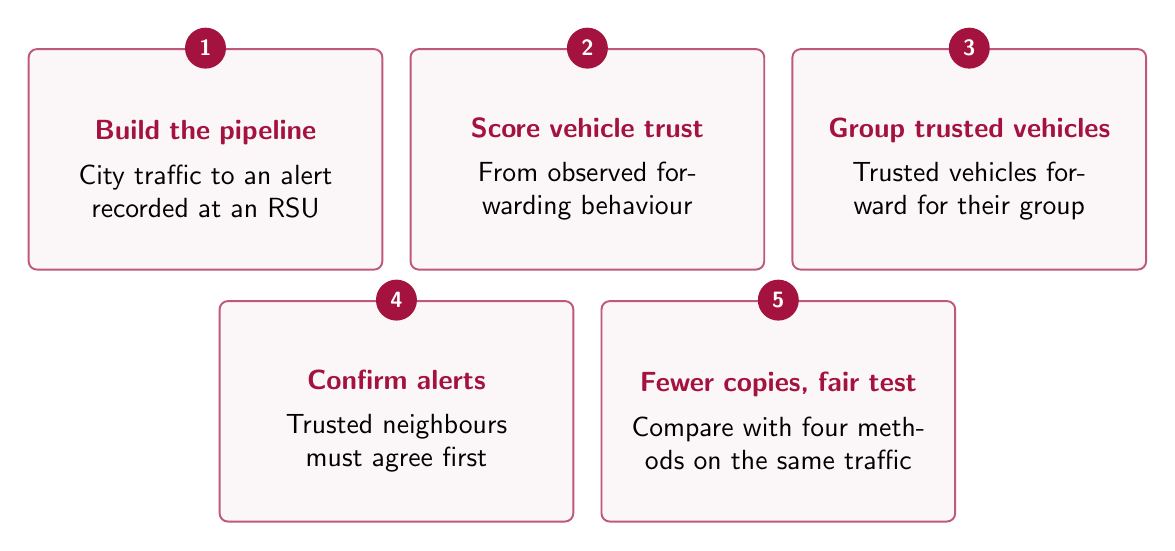
\begin{tikzpicture}[x=1cm,y=1cm]
        \foreach \i/\x/\y/\t/\b in {
            1/0/0/{Build the pipeline}/{City traffic to an alert recorded at an RSU},
            2/4.85/0/{Score vehicle trust}/{From observed forwarding behaviour},
            3/9.7/0/{Group trusted vehicles}/{Trusted vehicles forward for their group},
            4/2.425/-3.2/{Confirm alerts}/{Trusted neighbours must agree first},
            5/7.275/-3.2/{Fewer copies, fair test}/{Compare with four methods on the same traffic}}{
            \node[objective] (o\i) at (\x,\y) {\mbox{}\\[2pt]{\color{amritaMaroon}\textbf{\t}}\\[4pt]\b};
            \node[num=amritaMaroon] at (o\i.north) {\i};}
    \end{tikzpicture}
\end{frame}

% =========================================================================
\section{Proposed System}

\begin{frame}{10. Proposed Solution}
    \centering
    \vspace{0.3cm}
    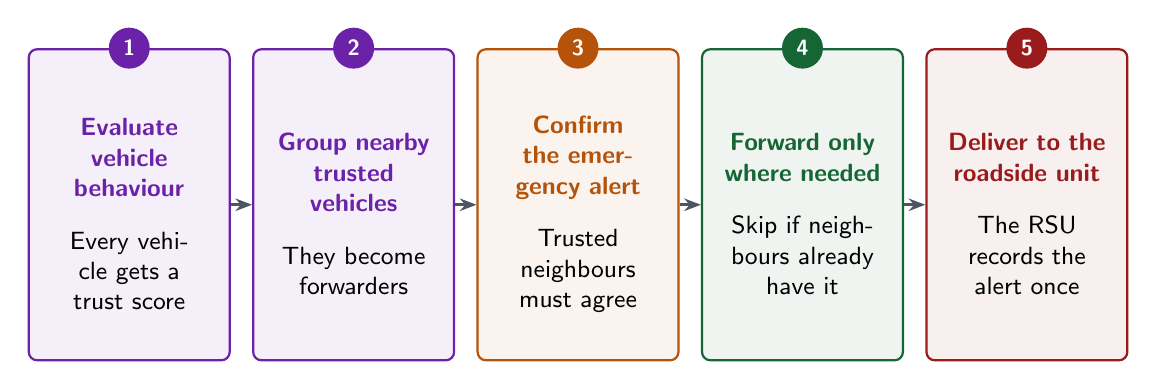
\begin{tikzpicture}[x=1cm,y=1cm]
        \foreach \i/\x/\c/\t/\b in {
            1/0/cTrust/{Evaluate vehicle behaviour}/{Every vehicle gets a trust score},
            2/2.85/cTrust/{Group nearby trusted vehicles}/{They become forwarders},
            3/5.7/cVerify/{Confirm the emergency alert}/{Trusted neighbours must agree},
            4/8.55/cDissem/{Forward only where needed}/{Skip if neighbours already have it},
            5/11.4/cRSU/{Deliver to the roadside unit}/{The RSU records the alert once}}{
            \node[idea=\c] (b\i) at (\x,0) {\mbox{}\\[2pt]{\color{\c}\textbf{\t}}\\[8pt]\b};
            \node[num=\c] at (b\i.north) {\i};}
        \foreach \a/\b in {1/2,2/3,3/4,4/5} \draw[flow] (b\a.east) -- (b\b.west);
    \end{tikzpicture}
    \takeaway{The alert spreads with far fewer copies, and only after trusted vehicles confirm it.}
\end{frame}

\begin{frame}{11. System Architecture}
    \centering
    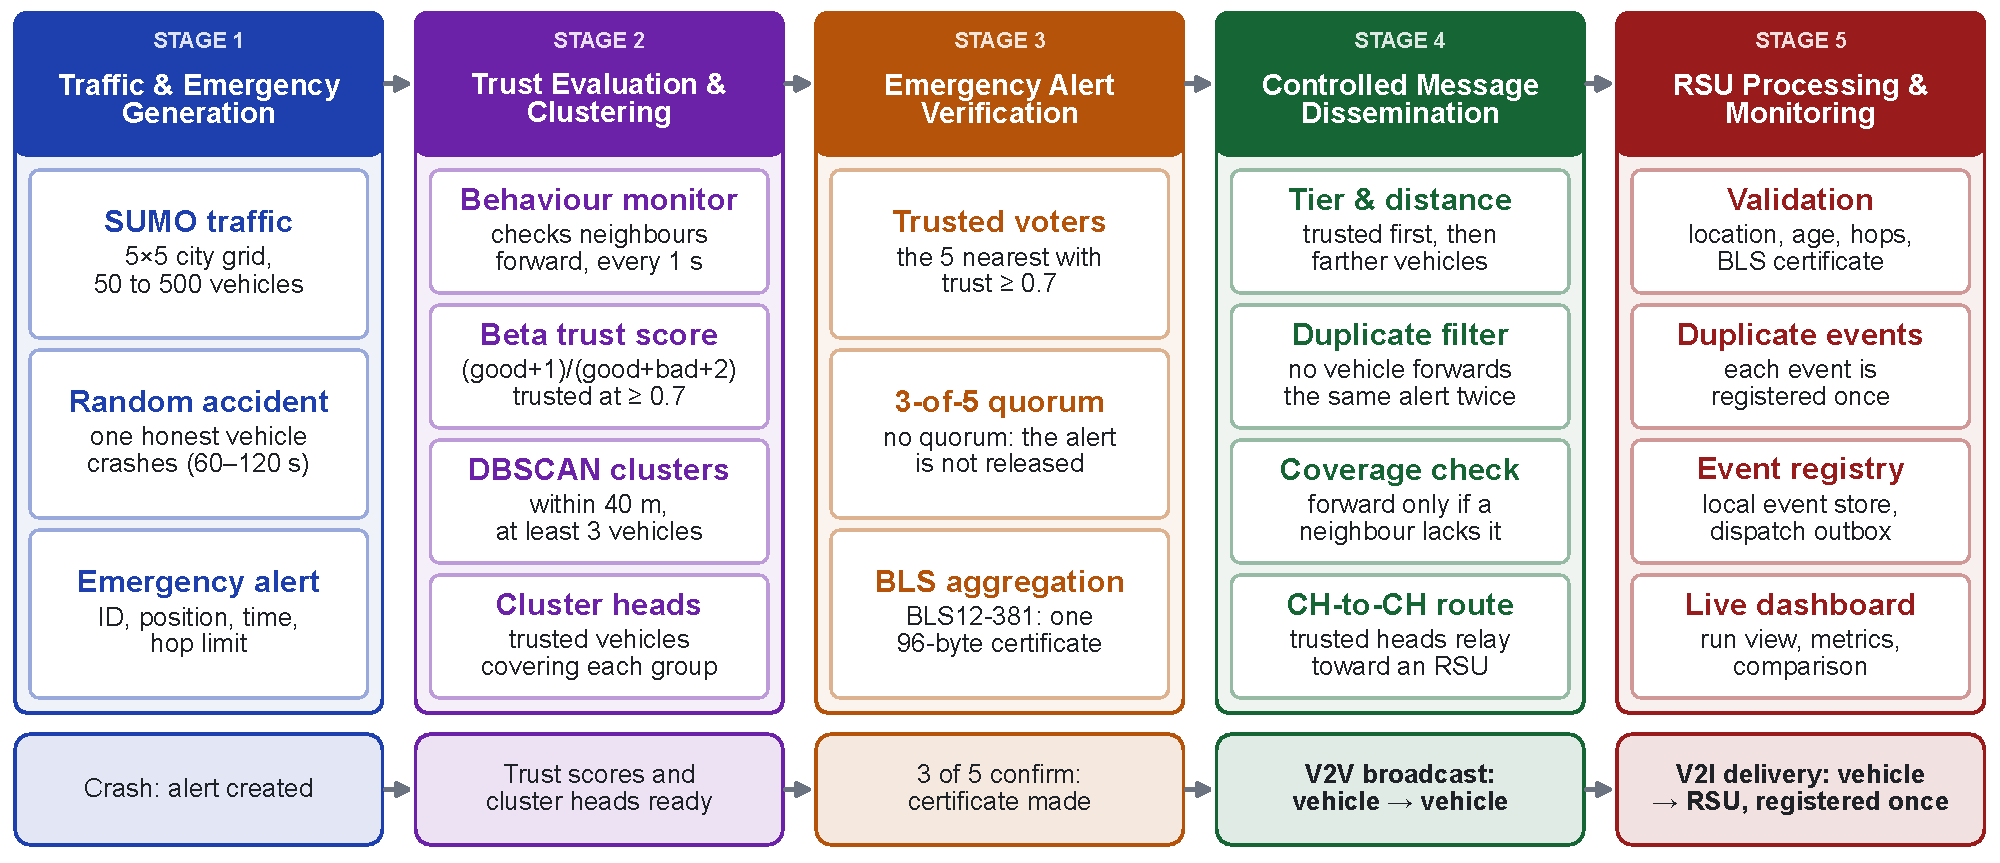
\includegraphics[width=\textwidth]{architecture/architecture_implemented.pdf}
    \shotcap{Implemented components only, checked against the source code. Algorithms: slide 17. Cloud integration
    is proposed future work (slide 21), not part of this system.}
\end{frame}

\begin{frame}{12. End-to-End Workflow: One Simulated Accident}
    \begin{columns}[c]
        \column{0.43\textwidth}
        \centering
        \annot{height=5.45cm}{view_map_walk_02_incident.png}{
            \draw[hl] (0.81,0.707) circle[radius=0.21cm];
            \node[call, anchor=north east] (c1) at (0.98,0.6) {accident};
            \draw[ptr] (c1.north) -- (0.81,0.672);
            \node[call, anchor=north] (c2) at (0.6,0.16) {RSU-2};
            \draw[ptr] (c2.north) -- (0.745,0.25);}
        \shotcap{Genuine SUMO-GUI capture \cite{lopez2018sumo}: city grid, 200 vehicles.}
        \column{0.55\textwidth}
        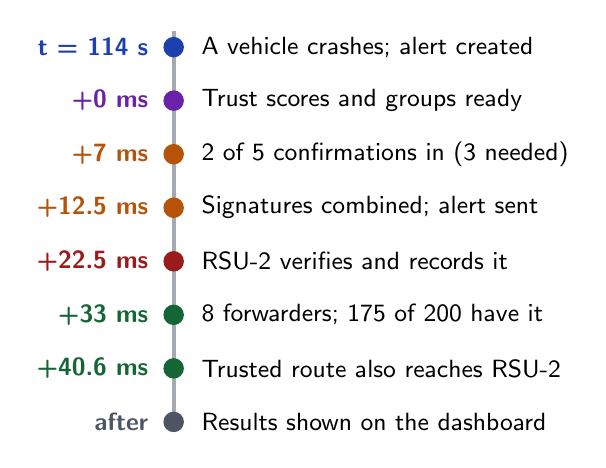
\begin{tikzpicture}[x=1cm,y=1cm]
            \draw[inkGray!50, line width=1.4pt] (1.95,-0.05) -- (1.95,-5.0);
            \foreach \i/\c/\tm/\ev in {
                0/cTraffic/{t = 114 s}/{A vehicle crashes; alert created},
                1/cTrust/{+0 ms}/{Trust scores and groups ready},
                2/cVerify/{+7 ms}/{2 of 5 confirmations in (3 needed)},
                3/cVerify/{+12.5 ms}/{Signatures combined; alert sent},
                4/cRSU/{+22.5 ms}/{RSU-2 verifies and records it},
                5/cDissem/{+33 ms}/{8 forwarders; 175 of 200 have it},
                6/cDissem/{+40.6 ms}/{Trusted route also reaches RSU-2},
                7/inkGray/{after}/{Results shown on the dashboard}}{
                \pgfmathsetmacro{\yy}{-0.25-0.68*\i}
                \node[font=\small\bfseries, text=\c, anchor=east] at (1.75,\yy) {\tm};
                \node[circle, fill=\c, minimum size=0.26cm, inner sep=0pt] at (1.95,\yy) {};
                \node[font=\small, anchor=west] at (2.18,\yy) {\ev};}
        \end{tikzpicture}
    \end{columns}
    \takeaway{In this genuine run, the verified alert was recorded at the RSU 22.5 ms after the crash.}
\end{frame}

% =========================================================================
\section{Implementation}

\begin{frame}{13. Trust Evaluation and Vehicle Grouping}
    \begin{columns}[T]
        \column{0.43\textwidth}
        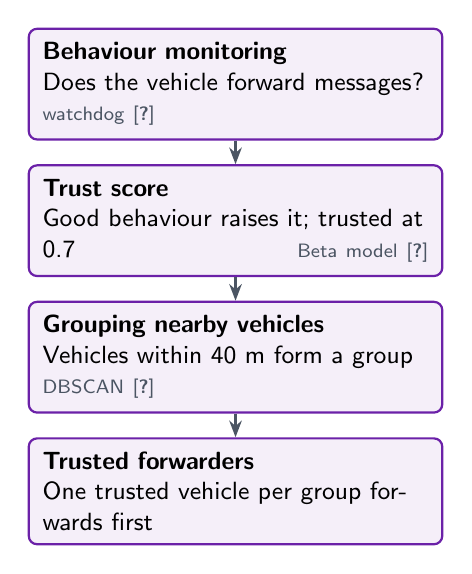
\begin{tikzpicture}[x=1cm,y=1cm]
            \node[step=cTrust] (s1) at (0,0) {\textbf{Behaviour monitoring}\\Does the vehicle forward messages?
                \hfill{\scriptsize\color{inkGray}watchdog \cite{marti2000watchdog}}};
            \node[step=cTrust, below=0.3cm of s1] (s2) {\textbf{Trust score}\\Good behaviour raises it; trusted at
                0.7 \hfill{\scriptsize\color{inkGray}Beta model \cite{josang2002beta}}};
            \node[step=cTrust, below=0.3cm of s2] (s3) {\textbf{Grouping nearby vehicles}\\Vehicles within 40 m form a
                group \hfill{\scriptsize\color{inkGray}DBSCAN \cite{ester1996dbscan}}};
            \node[step=cTrust, below=0.3cm of s3] (s4) {\textbf{Trusted forwarders}\\One trusted vehicle per group
                forwards first};
            \foreach \a/\b in {s1/s2,s2/s3,s3/s4} \draw[flow] (\a.south) -- (\b.north);
        \end{tikzpicture}
        \column{0.55\textwidth}
        \centering
        \annot{height=5.85cm}{view_map_walk_04_clusters.png}{
            \draw[hl] (0.735,0.425) circle[radius=0.2cm];
            \node[call, anchor=north] (c1) at (0.62,0.27) {trusted forwarder};
            \draw[ptr] (c1.north) -- (0.722,0.395);
            \draw[hl] (0.502,0.505) circle[radius=0.17cm];
            \node[call, anchor=south] (c2) at (0.36,0.62) {a group};
            \draw[ptr] (c2.south) -- (0.49,0.53);}
        \shotcap{Black rings: 20 trusted forwarders, one per group.}
    \end{columns}
\end{frame}

\begin{frame}{14. Alert Verification and Authentication}
    \centering
    {\large\textbf{Before an alert spreads, nearby trusted vehicles must confirm it.}}
    \par\vspace{0.3cm}
    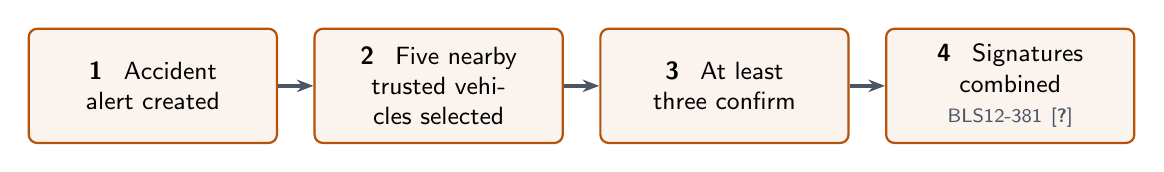
\begin{tikzpicture}[x=1cm,y=1cm, st/.style={tile=cVerify, font=\small, text width=2.8cm, minimum height=1.45cm}]
        \node[st] (a) at (0,0) {\textbf{1} \enspace Accident alert created};
        \node[st, right=0.45cm of a] (b) {\textbf{2} \enspace Five nearby trusted vehicles selected};
        \node[st, right=0.45cm of b] (c) {\textbf{3} \enspace At least three confirm};
        \node[st, right=0.45cm of c] (d) {\textbf{4} \enspace Signatures combined\\{\scriptsize\color{inkGray}BLS12-381
            \cite{boneh2004short}}};
        \foreach \x/\y in {a/b,b/c,c/d} \draw[flow] (\x) -- (\y);
    \end{tikzpicture}
    \par\vspace{0.25cm}
    \begin{minipage}[t]{0.47\textwidth}
        \centering
        \annot{height=3.75cm}{sl_zoom_votes.png}{
            \draw[hl] (0.4,0.51) circle[radius=0.3cm];
            \draw[hl] (0.665,0.51) circle[radius=0.3cm];
            \node[call, anchor=north] (c1) at (0.53,0.27) {confirmations arriving};
            \draw[ptr] (c1.north) -- (0.43,0.44);
            \draw[ptr] (c1.north) -- (0.64,0.44);}
        \shotcap{Step 3: 2 of 5 confirmations in (+7 ms)}
    \end{minipage}\hfill
    \begin{minipage}[t]{0.47\textwidth}
        \centering
        \annot{height=3.75cm}{sl_zoom_certificate.png}{
            \draw[hl] (0.532,0.51) circle[radius=0.32cm];
            \node[call, anchor=north] (c1) at (0.53,0.25) {verified alert sent};
            \draw[ptr] (c1.north) -- (0.532,0.43);}
        \shotcap{Step 4: one 96-byte certificate; receivers check it (+12.5 ms)}
    \end{minipage}
\end{frame}

\begin{frame}{15. Controlled Forwarding and RSU Delivery}
    \centering
    {\large\textbf{Forward the alert only when a nearby vehicle or RSU still needs it.}}
    \par\vspace{0.2cm}
    \begin{columns}[T]
        \column{0.36\textwidth}
        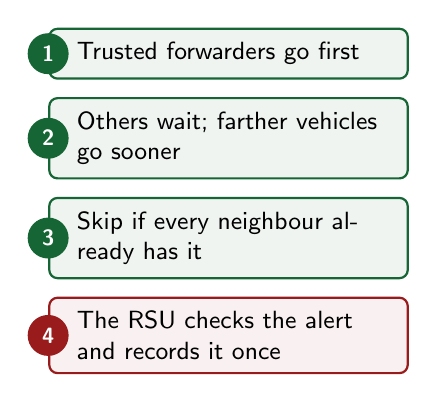
\begin{tikzpicture}[x=1cm,y=1cm, st/.style={tile=cDissem, text width=3.85cm, align=left, font=\small,
            anchor=north west, inner xsep=10pt}]
            \node[st] (r1) at (0.3,0) {Trusted forwarders go first};
            \node[st, below=0.22cm of r1] (r2) {Others wait; farther vehicles go sooner};
            \node[st, below=0.22cm of r2] (r3) {Skip if every neighbour already has it};
            \node[st, draw=cRSU, fill=cRSU!6, below=0.22cm of r3] (r4) {The RSU checks the alert and records it
                once};
            \foreach \i in {1,2,3} \node[num=cDissem] at (r\i.west) {\i};
            \node[num=cRSU] at (r4.west) {4};
        \end{tikzpicture}
        \column{0.62\textwidth}
        \centering
        \begin{minipage}[t]{0.49\linewidth}
            \centering
            {\small\textbf{Blind flooding}}\\[2pt]
            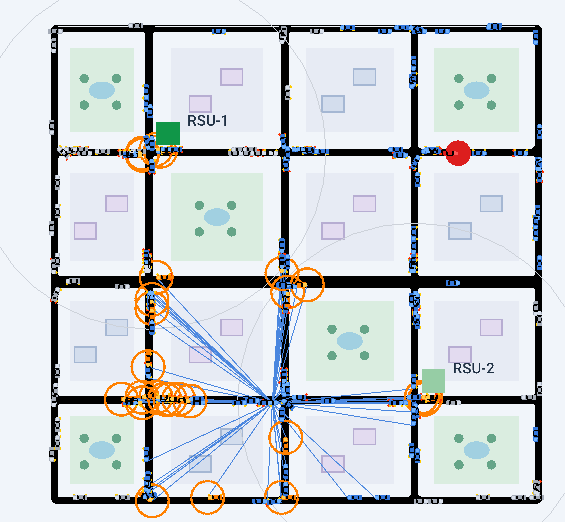
\includegraphics[width=0.95\linewidth]{view_map_walk_07_flooding.png}
            \shotcap{89 vehicles resend\\3380 lost receptions}
        \end{minipage}\hfill
        \begin{minipage}[t]{0.49\linewidth}
            \centering
            {\small\textbf{Proposed}}\\[2pt]
            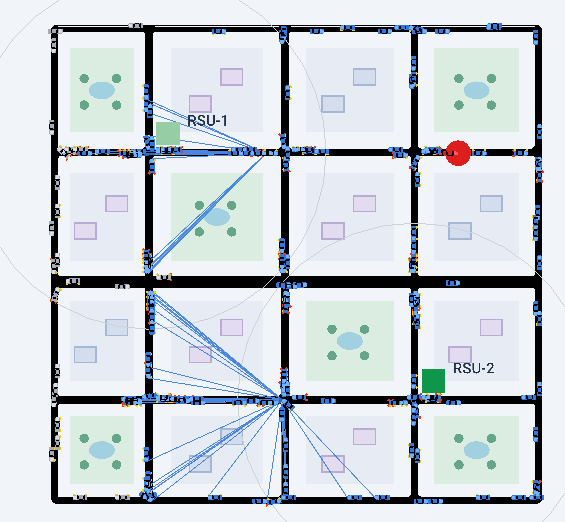
\includegraphics[width=0.95\linewidth]{view_map_walk_09_duplicates.png}
            \shotcap{8 vehicles resend\\78 lost receptions}
        \end{minipage}
        \par\vspace{2pt}
        {\footnotesize\color{inkGray} One run each (illustration). Orange rings: senders.\par}
    \end{columns}
\end{frame}

% =========================================================================
\section{Evaluation}

\begin{frame}{16. Four Baselines and the Proposed Method}
    \centering
    \renewcommand{\arraystretch}{1.38}
    \begin{tabular}{@{}>{\raggedright\arraybackslash}p{5.5cm}>{\raggedright\arraybackslash}p{8.0cm}@{}}
        \toprule
        \textbf{Approach} & \textbf{How it forwards the alert} \\
        \midrule
        Blind flooding & Every accepting vehicle forwards immediately \\
        Flooding + random delay \cite{ni1999broadcast} & Vehicles wait briefly (0--5 ms), then forward \\
        Slotted 1-persistence \cite{wisitpongphan2007} & Farther vehicles go first; a heard duplicate cancels \\
        \rowcolor{rowBase}\textbf{Slotted 1-p + random delay}\newline{\footnotesize\textbf{\color{baseBlue}strongest
            baseline}} & Distance slots plus a short random delay \\
        \rowcolor{rowProp}\textbf{\color{amritaMaroon}Proposed} & Trusted vehicles first; forward only if a neighbour
            lacks the alert \\
        \bottomrule
    \end{tabular}
    \takeaway{The baselines are our implementations of known rules. All five share trust scores, alert confirmation and
    RSU checks: \textbf{only the forwarding rule differs}.}
\end{frame}

\begin{frame}{17. Algorithms Used and Our Improvements}
    \centering
    \footnotesize
    \setlength{\tabcolsep}{4pt}
    \renewcommand{\arraystretch}{1.22}
    \begin{tabular}{@{}>{\raggedright\arraybackslash}p{2.75cm}>{\raggedright\arraybackslash}p{4.9cm}>{\raggedright\arraybackslash}p{2.75cm}>{\raggedright\arraybackslash}p{2.75cm}@{}}
        \toprule
        \textbf{Technique} & \textbf{How it works} & \textbf{Existing use} & \textbf{Our improvement} \\
        \midrule
        \textbf{Vehicle trust score}\newline{\scriptsize\color{inkGray}Beta model \cite{josang2002beta}} &
            trust $=(s{+}1)/(s{+}f{+}2)$; $s$, $f$ = good and bad forwards seen; starts at 0.5, trusted at $\geq 0.7$ &
            suppression trusts any sender \cite{ni1999broadcast,wisitpongphan2007} &
            only trusted vehicles lead and confirm \\
        \arrayrulecolor{inkGray!30}\hline\arrayrulecolor{black}
        \textbf{Grouping vehicles}\newline{\scriptsize\color{inkGray}DBSCAN \cite{ester1996dbscan}} &
            vehicles within 40 m form a group of at least 3 &
            groups for network stability \cite{chen2024dnov} &
            one trusted forwarder per group \\
        \arrayrulecolor{inkGray!30}\hline\arrayrulecolor{black}
        \textbf{Neighbour confirmation} &
            the 5 nearest trusted neighbours vote; at least 3 must agree &
            a signature proves only the sender \cite{zhang2008batch} &
            no single vehicle can start an alert \\
        \arrayrulecolor{inkGray!30}\hline\arrayrulecolor{black}
        \textbf{Combining signatures}\newline{\scriptsize\color{inkGray}BLS12-381 \cite{boneh2004short}} &
            all signatures merge into one 96-byte certificate &
            signatures verified in batches \cite{zhang2008batch} &
            one small certificate, checked once \\
        \arrayrulecolor{inkGray!30}\hline\arrayrulecolor{black}
        \textbf{Controlled broadcast} &
            wait = tier (25 ms) + distance slot (0--20 ms) + 0--5 ms; forward only if a neighbour lacks it &
            farther first; a duplicate cancels \cite{wisitpongphan2007} &
            trusted vehicles first; covered areas stay silent \\
        \arrayrulecolor{inkGray!30}\hline\arrayrulecolor{black}
        \textbf{Trusted route to RSU} &
            shortest path over trusted forwarders; each confirms locally &
            route by travel direction \cite{kaur2024route} &
            a second, verified path to the RSU \\
        \bottomrule
    \end{tabular}
\end{frame}

\begin{frame}{18. Experimental Setup}
    \centering
    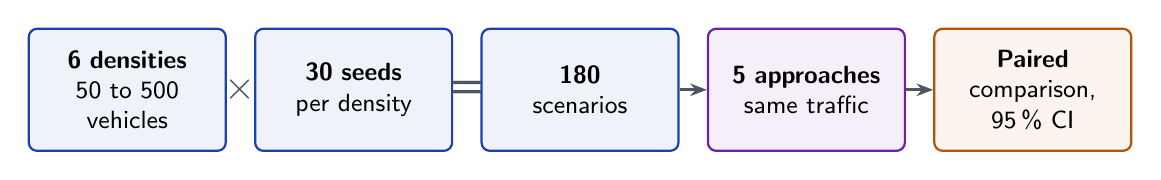
\begin{tikzpicture}[x=1cm,y=1cm]
        \node[pipe=cTraffic, text width=2.15cm] (a) at (1.2,0) {\textbf{6 densities}\\50 to 500 vehicles};
        \node[pipe=cTraffic, text width=2.15cm] (b) at (4.075,0) {\textbf{30 seeds}\\per density};
        \node[pipe=cTraffic, text width=2.15cm] (c) at (6.95,0) {\textbf{180}\\scenarios};
        \node[pipe=cTrust, text width=2.15cm] (d) at (9.825,0) {\textbf{5 approaches}\\same traffic};
        \node[pipe=cVerify, text width=2.15cm] (e) at (12.7,0) {\textbf{Paired}\\comparison, 95\,\% CI};
        \node[font=\Large\bfseries, text=inkGray] at (2.6375,0) {$\times$};
        \node[font=\Large\bfseries, text=inkGray] at (5.5125,0) {=};
        \draw[flow] (c) -- (d);
        \draw[flow] (d) -- (e);
    \end{tikzpicture}
    \par\vspace{0.2cm}
    {\small SUMO $5\times5$ city grid \;$\cdot$\; 2 RSUs at junctions \cite{trullols2010rsu}\\
    10\,\% misbehaving vehicles \;$\cdot$\; 802.11p radio \cite{ieee80211p}\par}
    \par\vspace{0.4cm}
    {\large\textbf{\color{amritaMaroon}What we measure for each alert}}\par\vspace{0.2cm}
    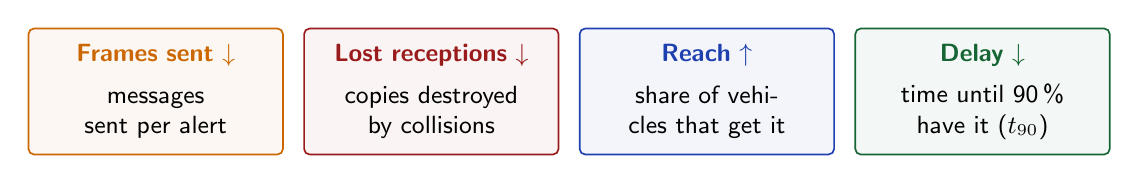
\begin{tikzpicture}[x=1cm,y=1cm]
        \foreach \i/\c/\t/\d in {
            0/orange!80!black/{Frames sent $\downarrow$}/{messages sent per alert},
            1/cRSU/{Lost receptions $\downarrow$}/{copies destroyed by collisions},
            2/cTraffic/{Reach $\uparrow$}/{share of vehicles that get it},
            3/cDissem/{Delay $\downarrow$}/{time until 90\,\% have it ($t_{90}$)}}{
            \node[metric=\c, text width=2.95cm, minimum height=1.6cm] at (3.5*\i,0)
                {{\color{\c}\textbf{\t}}\\[4pt]\d};}
    \end{tikzpicture}
\end{frame}

\begin{frame}{19. Results and Performance Comparison}
    \centering
    {\small\renewcommand{\arraystretch}{1.06}\gentable{tab_slide_results.tex}}
    \shotcap{200 vehicles $\cdot$ mean $\pm$ 95\,\% CI over 30 paired runs $\cdot$ bold: best mean $\cdot$ blue row:
    strongest baseline}
    \begin{columns}[T]
        \column{0.38\textwidth}
        \centering
        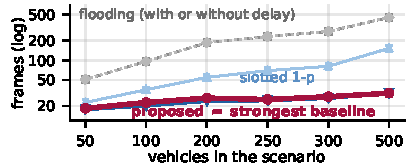
\includegraphics[width=\linewidth]{sl_frames_density.pdf}
        \column{0.60\textwidth}
        \small
        \begin{itemize}\setlength{\itemsep}{1pt}
            \item[\textcolor{amritaMaroon}{\textbullet}] \textbf{\color{amritaMaroon}Fewest mean lost receptions:}
                  \NLossProp{} vs \NLossSlotRad{} (not significant)
            \item[\textcolor{baseBlue}{\textbullet}] \textbf{\color{baseBlue}Frames close to strongest baseline:}
                  \NFrProp{} vs \NFrSlotRad{}
            \item[\textcolor{inkGray}{\textbullet}] \textbf{Trade-off:} delay slightly higher, \NTnProp{} vs
                  \NTnSlotRad{}~ms (\NDTnSlotRadFiveH{}~ms at 500 vehicles)
        \end{itemize}
    \end{columns}
    \takeaway{\textbf{The proposed method achieved a measured reach of \NReachProp\,\% across 30 runs at 200 vehicles.}
    This is an experimental observation under the tested simulation conditions, not a guarantee of complete delivery.}
\end{frame}

\begin{frame}{20. Security Evaluation, Trade-offs and Limitations}
    \begin{columns}[T]
        \column{0.46\textwidth}
        \centering
        {\small\textbf{Forged alerts recorded by an RSU}}\par\vspace{2pt}
        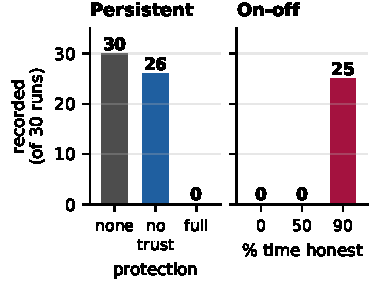
\includegraphics[width=0.94\linewidth]{sl_forgery.pdf}
        \shotcap{200 vehicles, 30 runs per bar.\\Security has a price: confirming every alert adds about \NSecTn{} ms of
        delay.}
        \column{0.52\textwidth}
        \point{cDissem}{Stops persistent attackers}{With full protection, 0 of 30 forged alerts were recorded.}
        \point{cRSU}{Weakness: on-off attackers}{Vehicles honest 90\,\% of the time still earn trust: 25 of 30
        recorded.}
        \point{cVerify}{Sparse traffic}{Too few trusted neighbours: no alert sent (14 of 30 at 50 vehicles, 150 m).}
        \point{inkGray}{Simulation only}{Idealised radio, small grid; keys from vehicle IDs, no PKI.}
    \end{columns}
\end{frame}

% =========================================================================
\section{Conclusion}

\begin{frame}{21. Conclusion and Future Scope}
    \begin{columns}[T]
        \column{0.58\textwidth}
        {\large\textbf{\color{amritaMaroon}What we showed}}
        \begin{itemize}\setlength{\itemsep}{5pt}
            \item A complete, working pipeline: city traffic to an alert recorded at an RSU
            \item \NCutVsFlood\,\% fewer frames than blind flooding at 200 vehicles, similar measured reach
            \item Fewer lost receptions (dense) and more reach (sparse) than the strongest baseline
            \item The strongest baseline sends slightly fewer frames and is faster in dense traffic
        \end{itemize}
        \column{0.4\textwidth}
        {\large\textbf{\color{cTraffic}Future scope}}
        \begin{itemize}\setlength{\itemsep}{5pt}
            \item Trust that resists on-off attackers; a real key system
            \item Realistic radio and real road maps
            \item A fallback when too few trusted neighbours exist
            \item \textbf{Cloud integration}: proposed, not yet implemented
        \end{itemize}
    \end{columns}
    \takeaway{\textbf{Conclusion:} trusted, controlled forwarding greatly reduces the broadcast storm; it costs a few
    milliseconds, and its security is only as strong as the trust score.}
\end{frame}

\begin{frame}{22. Project Deliverables and Technical Enrichment Activities}
    \centering
    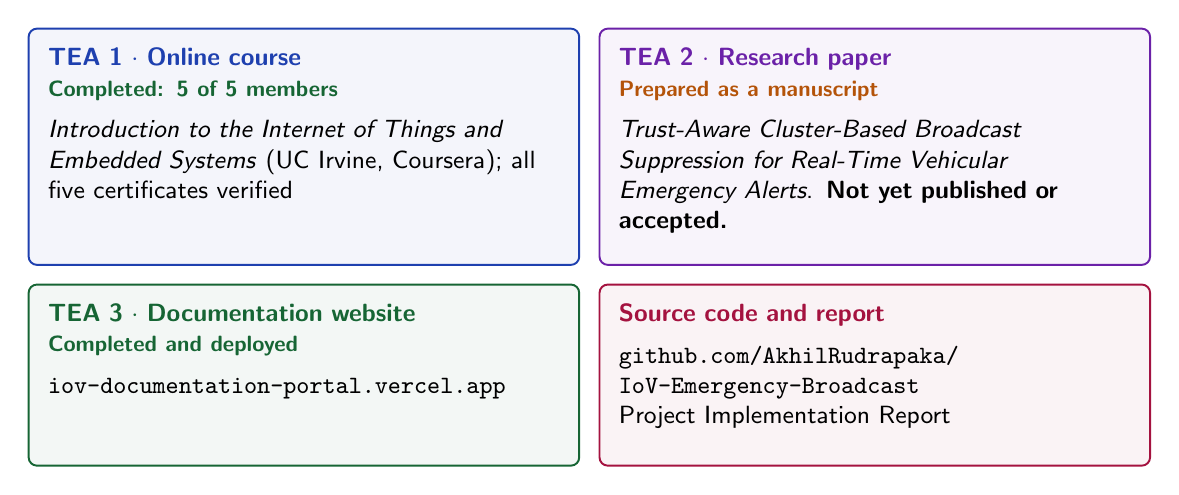
\begin{tikzpicture}[x=1cm,y=1cm]
        \node[quad=cTraffic, minimum height=3.0cm] at (0,0) {\parbox[t][2.5cm][t]{\linewidth}{\raggedright \textbf{\color{cTraffic}TEA 1 $\cdot$ Online course}\\
            {\footnotesize\color{cDissem}\textbf{Completed: 5 of 5 members}}\\[4pt]
            \emph{Introduction to the Internet of Things and Embedded Systems} (UC Irvine, Coursera); all five
            certificates verified}};
        \node[quad=cTrust, minimum height=3.0cm] at (7.25,0) {\parbox[t][2.5cm][t]{\linewidth}{\raggedright \textbf{\color{cTrust}TEA 2 $\cdot$ Research paper}\\
            {\footnotesize\color{cVerify}\textbf{Prepared as a manuscript}}\\[4pt]
            \emph{Trust-Aware Cluster-Based Broadcast Suppression for Real-Time Vehicular Emergency Alerts}.
            \textbf{Not yet published or accepted.}}};
        \node[quad=cDissem, minimum height=2.3cm] at (0,-3.25) {\parbox[t][1.8cm][t]{\linewidth}{\raggedright \textbf{\color{cDissem}TEA 3 $\cdot$ Documentation
            website}\\ {\footnotesize\color{cDissem}\textbf{Completed and deployed}}\\[4pt]
            \texttt{iov-documentation-portal.vercel.app}}};
        \node[quad=amritaMaroon, minimum height=2.3cm] at (7.25,-3.25) {\parbox[t][1.8cm][t]{\linewidth}{\raggedright \textbf{\color{amritaMaroon}Source code and
            report}\\[4pt] \texttt{github.com/AkhilRudrapaka/}\\\texttt{IoV-Emergency-Broadcast}\\
            Project Implementation Report}};
    \end{tikzpicture}
\end{frame}

% =========================================================================
\section{References}
\nocite{*}
\begin{frame}[allowframebreaks]{References}
    \fontsize{7.6}{8.9}\selectfont
    \bibliographystyle{ieeetr}
    \bibliography{references}
\end{frame}

\begin{frame}
    \centering
    
\includegraphics[width=2.6cm]{logo.png}\par\vspace{0.3cm}
    {\Huge \textbf{\textcolor{amritaMaroon}{Thank You}}}\par\vspace{0.2cm}
    {\large \textbf{Questions \& Viva Voce}}\par\vspace{0.25cm}
    {\color{amritaMaroon}\rule{0.55\textwidth}{0.8pt}}\par\vspace{0.2cm}
    {\small \textbf{Emergency Message Dissemination for Broadcast Storm Mitigation\\in the Internet of Vehicles}}
    \par\vspace{0.1cm}
    {\small Team \TeamNumber \quad | \quad Guide: \GuideName}\par\vspace{0.05cm}
    {\small \GuideDesignation, \GuideInstitution}
\end{frame}

\end{document}
